\documentclass[a4paper,12pt]{article}
\usepackage[brazil]{babel}
\usepackage[utf8]{inputenc}
\usepackage{amsmath,amssymb}
\usepackage[a4paper,margin=0.8in]{geometry}
\usepackage{enumerate}
\usepackage{multicol}
\usepackage{tikz}
\usetikzlibrary{patterns}



\begin{document}

\title{Quizz 3 - Uncertainty}
\author{BCC325 - Intelligência Artificial}
\date{}
\maketitle

\section*{Questão 1}

Considere um baralho padrão de 52 cartas, com 13 valores (Ás, Rei, Rainha, Valete e os números de 2 a 10) em cada um dos quatro naipes (paus, ouros, copas e espadas). Se uma carta for sorteada aleatoriamente, qual é a probabilidade de que seja uma carta de espadas ou um dois? Apresente os cálculos e deixe claro o raciocínio. Respostas sem apresentação dos cálculos e raciocínio não serão consideradas.

\textbf{Nota:} O "ou" nesta questão é inclusivo, ou seja, considera qualquer uma das condições satisfeitas.
    
\begin{multicols}{3}
\begin{enumerate}[a)]
    \item Aproximadamente 0,019
    \item Aproximadamente 0,077
    \item Aproximadamente 0,17
    \item Aproximadamente 0,25
    \item Aproximadamente 0,308
    \item Aproximadamente 0,327
    \item Aproximadamente 0,5
    \item Nenhuma das opções acima
\end{enumerate}
\end{multicols}


\section*{Questão 2}

Imagine lançar duas moedas justas, onde cada moeda tem um lado "Cara" e um lado "Coroa", com "Cara" aparecendo 50\% das vezes e "Coroa" aparecendo 50\% das vezes. Qual é a probabilidade de que, após lançar as duas moedas, uma delas caia em "Cara" e a outra em "Coroa"? Apresente os cálculos e deixe claro o raciocínio. Respostas sem apresentação dos cálculos e raciocínio não serão consideradas.

\section*{Questão 3}

Duas fábricas — Fábrica A e Fábrica B — produzem baterias para serem usadas em telefones celulares. A Fábrica A produz 60\% de todas as baterias, e a Fábrica B produz os outros 40\%. 2\% das baterias da Fábrica A apresentam defeitos, e 4\% das baterias da Fábrica B apresentam defeitos. Qual é a probabilidade de que uma bateria seja \textbf{tanto produzida pela Fábrica A quanto defeituosa}? Apresente os cálculos e deixe claro o raciocínio. Respostas sem apresentação dos cálculos e raciocínio não serão consideradas.

\begin{multicols}{3}
\begin{enumerate}[a)]
    \item 0,008
    \item 0,012
    \item 0,02
    \item 0,024
    \item 0,028
    \item 0,06
    \item 0,12
    \item 0,2
    \item 0,429
    \item 0,6
    \item Nenhuma das opções acima
\end{enumerate}
\end{multicols}

\pagebreak

\section*{Questão 4}

Considere a Rede Bayesiana mostrada na aula, reproduzida abaixo.

\begin{figure}[!ht]
    \centering
    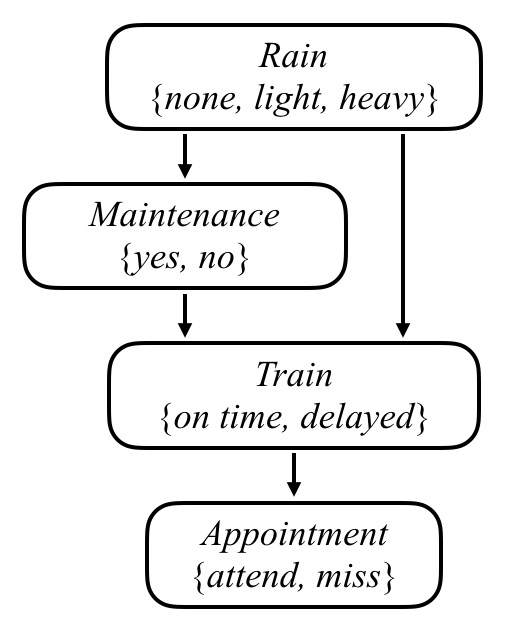
\includegraphics[width=0.4\textwidth]{bayesiannet.jpg}
\end{figure}

Qual das seguintes sentenças é verdadeira?

\begin{enumerate}[a)]
    \item Assumindo que sabemos que o trem está no horário, se está chovendo ou não afeta a probabilidade de que o compromisso seja atendido.
    \item Assumindo que sabemos que está chovendo, se há manutenção nos trilhos ou não \textbf{não} afeta a probabilidade de que o trem esteja no horário.
    \item Assumindo que sabemos que há manutenção nos trilhos, se está chovendo ou não \textbf{não} afeta a probabilidade de que o trem esteja no horário.
    \item Assumindo que sabemos que o trem está no horário, se há manutenção nos trilhos ou não \textbf{não} afeta a probabilidade de que o compromisso seja atendido.
    \item Assumindo que sabemos que há manutenção nos trilhos, se está chovendo ou não \textbf{não} afeta a probabilidade de que o compromisso seja atendido.
\end{enumerate}

\section*{Questão 5}

Considere a sua implementação no arquivo heredity.py e responda:

\begin{enumerate} [a)]
    \item Como é calculada a probabilidade de um pai passar uma cópia do gene GJB2 se ele temduas cópias do gene? Em qual linha do código esse cálculo é feito?
    \item Como é calculada a probabilidade de um filho receber duas cópias do gene GJB2? Qual linha do seu código implementa essa operação? Explique a expressão?
    \item Qual é o código em python para se obter a probabilidade de uma pessoa ter problemas auditivos dado que ela tem 0 cópias do gene? De acordo com o código, qual seria essa probabilidade?
\end{enumerate}

\section*{Questão 6}

Considere a sua implementação no arquivo pagerank.py e responda:

\begin{enumerate} [a)]
    \item Como a função \texttt{transition\_model} distribui a probabilidade entre as páginas quando a página atual possui links de saída? Em que linha do código esse cálculo é feito?
    \item Qual é a equação usada para atualizar o PageRank de uma página na abordagem iterativa? Em que linha do código esse cálculo é implementado?
    \item Qual é o código em Python para obter a probabilidade de uma página ser escolhida inicialmente na abordagem de amostragem? Para um corpus com $N$ páginas, qual seria essa probabilidade de seleção?
\end{enumerate}





\end{document}
